% questions.tex —— 2012 年·江苏卷 · 题目内容片段（无答案）
% 由 tools/generate_projects.py 依来源总账自 2012/2012_数学真题_江苏_试题.md 生成，勿手改（改源 MD 后重跑）


\begin{gknotice}
\textbf{来源说明}：本题面依据固定源 PDF 的两页 A3 题面逐题转录。第 745 面为填空题 1—14 与解答题 15—18，第 746 面为解答题 19—20 与附加题 21—23；原卷第 746 面直接续排 21—23，未另设“附加题”标题，本稿按江苏卷通例归入“三、附加题”。第 21 题为四选二（A 几何证明选讲、B 矩阵与变换、C 坐标系与参数方程、D 不等式选讲），四题全部收录，依次记为（1）—（4）并冠以【A】—【D】。

\textbf{解析归属}：固定源不附答案或解析；配套答案与解析均由本库按本题面独立复算（等级 D，非官方）。

\textbf{图形说明}：第 4 题算法流程图、第 7 题长方体、第 9 题矩形、第 16 题直三棱柱、第 17 题炮弹轨迹、第 19 题椭圆、第 21A 题圆，均由项目内 TikZ 矢量源重绘。
\end{gknotice}

\gkpart{一、填空题}

\begin{question}
\gkti{1}已知集合 $A=\{1,2,4\}$，$B=\{2,4,6\}$，则 $A\cup B=$ $\underline{\qquad}$。

\end{question}
\begin{question}
\gkti{2}某学校高一、高二、高三年级的学生人数之比是 $3:3:4$，现用分层抽样的方法从该校高中三个年级的学生中抽取容量为 $50$ 的样本，则应从高二年级抽取 $\underline{\qquad}$ 名学生。

\end{question}
\begin{question}
\gkti{3}设 $a$，$b\in\mathbf R$，$a+b\mathrm i=\dfrac{11-7\mathrm i}{1-2\mathrm i}$（$\mathrm i$ 为虚数单位），则 $a+b$ 的值为 $\underline{\qquad}$。

\Needspace{0.4\textheight}
\end{question}
\begin{question}
\gkti{4}如图是一个算法流程图，则输出的 $k$ 的值是 $\underline{\qquad}$。
\nopagebreak[4]
\begin{center}% ============================================================
% f2012_jiangsu_q04_flowchart.tex
% 2012 江苏卷第 4 题 算法流程图（TikZ 矢量重绘）
% 开始 → k←1 → 判断 k^2-5k+4>0；否：k←k+1 回代；是：输出 k → 结束
% ============================================================
\begin{tikzpicture}[
  x=1cm, y=1cm, line width=0.6pt, font=\footnotesize, >=Stealth,
  every node/.style={inner sep=3pt},
  proc/.style={rectangle, draw, minimum width=2.4cm, minimum height=0.62cm},
  io/.style={trapezium, draw, trapezium left angle=70, trapezium right angle=110,
             minimum width=2.8cm, minimum height=0.66cm},
  dec/.style={diamond, draw, aspect=2.6, minimum width=3.4cm, minimum height=0.95cm},
  term/.style={rectangle, rounded corners=8pt, draw, minimum width=2.0cm,
               minimum height=0.58cm}
]

  \node[term] (start) at (0,0) {开始};
  \node[proc] (init)  at (0,-1.35) {$k\leftarrow1$};
  \node[dec]  (judge) at (0,-2.95) {$k^2-5k+4>0$};
  \node[proc] (inc)   at (4.10,-2.95) {$k\leftarrow k+1$};
  \node[io]   (out)   at (0,-4.45) {输出 $k$};
  \node[term] (end)   at (0,-5.75) {结束};

  \draw[->] (start) -- (init);
  \draw[->] (init) -- (judge);
  \draw[->] (judge) -- (out);
  \node at (0.55,-3.62) {Y};
  \draw[->] (out) -- (end);
  \draw[->] (judge.east) -- node[above] {N} (inc.west);

  % 否：k←k+1 之后回到判断框之前
  \draw[->] (inc.north) -- (4.10,-1.95) -- (0,-1.95);

\end{tikzpicture}
\end{center}
\nopagebreak[4]
\end{question}
\begin{question}
\gkti{5}函数 $f(x)=\sqrt{1-2\log_6x}$ 的定义域为 $\underline{\qquad}$。

\end{question}
\begin{question}
\gkti{6}现有 $10$ 个数，它们能构成一个以 $1$ 为首项，$-3$ 为公比的等比数列，若从这 $10$ 个数中随机抽取一个数，则它小于 $8$ 的概率是 $\underline{\qquad}$。

\Needspace{0.4\textheight}
\end{question}
\begin{question}
\gkti{7}如图，在长方体 $ABCD-A_1B_1C_1D_1$ 中，$AB=AD=3$ cm，$AA_1=2$ cm，则四棱锥 $A-BB_1D_1D$ 的体积为 $\underline{\qquad}$ cm$^3$。
\nopagebreak[4]
\begin{center}% ============================================================
% f2012_jiangsu_q07_cuboid.tex
% 2012 江苏卷第 7 题 长方体 ABCD-A1B1C1D1 与四棱锥 A-BB1D1D
% AB=AD=3 cm，AA1=2 cm（TikZ 矢量重绘）
% ============================================================
\begin{tikzpicture}[x=1cm, y=1cm, line width=0.6pt, font=\footnotesize]

  \coordinate (A)  at (0,0);
  \coordinate (B)  at (3.0,0);
  \coordinate (C)  at (4.2,1.15);
  \coordinate (D)  at (1.2,1.15);
  \coordinate (A1) at (0,1.85);
  \coordinate (B1) at (3.0,1.85);
  \coordinate (C1) at (4.2,3.00);
  \coordinate (D1) at (1.2,3.00);

  % ---------- 长方体的棱 ----------
  \draw (A) -- (B) -- (C);
  \draw[dashed] (C) -- (D) -- (A);
  \draw (A) -- (A1);
  \draw (B) -- (B1);
  \draw (C) -- (C1);
  \draw[dashed] (D) -- (D1);
  \draw (A1) -- (B1) -- (C1) -- (D1) -- cycle;

  % ---------- 四棱锥 A-BB1D1D ----------
  \draw (B) -- (B1);
  \draw (B1) -- (D1);
  \draw[dashed] (D1) -- (D);
  \draw[dashed] (D) -- (B);
  \draw (A) -- (B1);
  \draw[dashed] (A) -- (D1);

  % ---------- 标注 ----------
  \node[below left]  at (A)  {$A$};
  \node[below]       at (B)  {$B$};
  \node[right]       at (C)  {$C$};
  \node at ($(D)+(-0.34,0.24)$) {$D$};
  \node[left]        at (A1) {$A_1$};
  \node[right]       at (B1) {$B_1$};
  \node[above right] at (C1) {$C_1$};
  \node[above]       at (D1) {$D_1$};

\end{tikzpicture}
\end{center}
\nopagebreak[4]
\end{question}
\begin{question}
\gkti{8}在平面直角坐标系 $xOy$ 中，若双曲线 $\dfrac{x^2}{m}-\dfrac{y^2}{m^2+4}=1$ 的离心率为 $\sqrt5$，则 $m$ 的值为 $\underline{\qquad}$。

\Needspace{0.4\textheight}
\end{question}
\begin{question}
\gkti{9}如图，在矩形 $ABCD$ 中，$AB=\sqrt2$，$BC=2$，点 $E$ 为 $BC$ 的中点，点 $F$ 在边 $CD$ 上，若 $\overrightarrow{AB}\cdot\overrightarrow{AF}=\sqrt2$，则 $\overrightarrow{AE}\cdot\overrightarrow{BF}$ 的值是 $\underline{\qquad}$。
\nopagebreak[4]
\begin{center}% ============================================================
% f2012_jiangsu_q09_rectangle.tex
% 2012 江苏卷第 9 题 矩形 ABCD，E 为 BC 中点，F 在边 CD 上
% AB=√2，BC=2；图中标出向量 AB、AF、AE（TikZ 矢量重绘）
% ============================================================
\begin{tikzpicture}[x=1cm, y=1cm, line width=0.6pt, font=\footnotesize, >=Stealth]

  \coordinate (A) at (0,0);
  \coordinate (B) at (2.20,0);
  \coordinate (C) at (2.20,3.10);
  \coordinate (D) at (0,3.10);
  \coordinate (E) at (2.20,1.55);
  \coordinate (F) at (1.556,3.10);

  % ---------- 矩形 ----------
  \draw (A) -- (B) -- (C) -- (D) -- cycle;

  % ---------- 向量 ----------
  \draw[->] (A) -- (B);
  \draw[->] (A) -- (F);
  \draw[->] (A) -- (E);

  % ---------- 标注 ----------
  \node[below left]  at (A) {$A$};
  \node[below right] at (B) {$B$};
  \node[right]       at (C) {$C$};
  \node[left]        at (D) {$D$};
  \node[right]       at (E) {$E$};
  \node[above]       at (F) {$F$};

\end{tikzpicture}
\end{center}
\nopagebreak[4]
\end{question}
\begin{question}
\gkti{10}设 $f(x)$ 是定义在 $\mathbf R$ 上且周期为 $2$ 的函数，且在区间 $[-1,1]$ 上，
\nopagebreak[4]
\[f(x)=\begin{cases}ax+1,&-1\leqslant x<0,\\[2pt]\dfrac{bx+2}{x+1},&0\leqslant x\leqslant1,\end{cases}\]
其中 $a$，$b\in\mathbf R$。若 $f\left(\dfrac12\right)=f\left(\dfrac32\right)$，则 $a+3b$ 的值为 $\underline{\qquad}$。

\end{question}
\begin{question}
\gkti{11}设 $\alpha$ 为锐角，若 $\cos\left(\alpha+\dfrac\pi6\right)=\dfrac45$，则 $\sin\left(2\alpha+\dfrac\pi{12}\right)$ 的值为 $\underline{\qquad}$。

\end{question}
\begin{question}
\gkti{12}在平面直角坐标系 $xOy$ 中，圆 $C$ 的方程为 $x^2+y^2-8x+15=0$，若直线 $y=kx-2$ 上至少存在一点，使得以该点为圆心，$1$ 为半径的圆与圆 $C$ 有公共点，则 $k$ 的最大值是 $\underline{\qquad}$。

\end{question}
\begin{question}
\gkti{13}已知函数 $f(x)=x^2+ax+b$（$a$，$b\in\mathbf R$）的值域为 $[0,+\infty)$，若关于 $x$ 的不等式 $f(x)<c$ 的解集为 $(m,m+6)$，则实数 $c$ 的值为 $\underline{\qquad}$。

\end{question}
\begin{question}
\gkti{14}已知正数 $a$，$b$，$c$ 满足 $5c-3a\leqslant b\leqslant4c-a$，$c\ln b\geqslant a+c\ln c$，则 $\dfrac ba$ 的取值范围是 $\underline{\qquad}$。

\end{question}
\gkpart{二、解答题}

\begin{question}
\gkti{15}在 $\triangle ABC$ 中，已知 $\overrightarrow{AB}\cdot\overrightarrow{AC}=3\overrightarrow{BA}\cdot\overrightarrow{BC}$。

（1） 求证：$\tan B=3\tan A$；

（2） 若 $\cos C=\dfrac{\sqrt5}5$，求 $A$ 的值。

\Needspace{0.4\textheight}
\end{question}
\begin{question}
\gkti{16}如图，在直三棱柱 $ABC-A_1B_1C_1$ 中，$A_1B_1=A_1C_1$，$D$，$E$ 分别是棱 $BC$，$CC_1$ 上的点（点 $D$ 不同于点 $C$），且 $AD\perp DE$，$F$ 为 $B_1C_1$ 的中点。求证：

（1） 平面 $ADE\perp$ 平面 $BCC_1B_1$；

（2） 直线 $A_1F\parallel$ 平面 $ADE$。
\nopagebreak[4]
\begin{center}% ============================================================
% f2012_jiangsu_q16_prism.tex
% 2012 江苏卷第 16 题 直三棱柱 ABC-A1B1C1（A1B1=A1C1）
% D 在棱 BC 上，E 在棱 CC1 上，F 为 B1C1 的中点（TikZ 矢量重绘）
% ============================================================
\begin{tikzpicture}[x=1cm, y=1cm, line width=0.6pt, font=\footnotesize]

  \coordinate (A)  at (0,0.60);
  \coordinate (B)  at (1.60,-0.50);
  \coordinate (C)  at (3.20,0.90);
  \coordinate (A1) at (0,3.60);
  \coordinate (B1) at (1.60,2.50);
  \coordinate (C1) at (3.20,3.90);
  \coordinate (D)  at (2.56,0.34);
  \coordinate (E)  at (3.20,1.90);
  \coordinate (F)  at (2.40,3.20);

  % ---------- 三棱柱的棱 ----------
  \draw (A) -- (B) -- (C);
  \draw[dashed] (C) -- (A);
  \draw (A) -- (A1);
  \draw (B) -- (B1);
  \draw (C) -- (C1);
  \draw (A1) -- (B1) -- (C1) -- cycle;

  % ---------- 题设线段 ----------
  \draw[dashed] (A) -- (D);
  \draw (D) -- (E);
  \draw (A1) -- (F);

  % ---------- 标注 ----------
  \node[below left]  at (A)  {$A$};
  \node[below]       at (B)  {$B$};
  \node[right]       at (C)  {$C$};
  \node[left]        at (A1) {$A_1$};
  \node[left]        at (B1) {$B_1$};
  \node[above right] at (C1) {$C_1$};
  \node at ($(D)+(-0.42,-0.10)$) {$D$};
  \node[right]       at (E)  {$E$};
  \node[above]       at (F)  {$F$};

\end{tikzpicture}
\end{center}
\nopagebreak[4]
\Needspace{0.4\textheight}
\end{question}
\begin{question}
\gkti{17}如图，建立平面直角坐标系 $xOy$，$x$ 轴在地平面上，$y$ 轴垂直于地平面，单位长度为 $1$ 千米，某炮位于坐标原点。已知炮弹发射后的轨迹在方程
\nopagebreak[4]
\[y=kx-\frac1{20}(1+k^2)x^2\qquad(k>0)\]
表示的曲线上，其中 $k$ 与发射方向有关。炮的射程是指炮弹落地点的横坐标。

（1） 求炮的最大射程；

（2） 设在第一象限有一飞行物（忽略其大小），其飞行高度为 $3.2$ 千米，试问它的横坐标 $a$ 不超过多少时，炮弹可以击中它？请说明理由。
\nopagebreak[4]
\begin{center}% ============================================================
% f2012_jiangsu_q17_trajectory.tex
% 2012 江苏卷第 17 题 炮弹抛物线轨迹（TikZ 矢量重绘）
% y=kx-(1/20)(1+k^2)x^2，图中画出一条典型轨迹
% ============================================================
\begin{tikzpicture}[x=1cm, y=1cm, line width=0.6pt, font=\footnotesize, >=Stealth]

  % ---------- 坐标轴 ----------
  \draw[->] (-0.3,0) -- (9.6,0) node[below] {$x$（千米）};
  \draw[->] (0,-0.3) -- (0,3.2) node[left] {$y$（千米）};
  \node[below left] at (0,0) {$O$};

  % ---------- 轨迹 ----------
  \draw[domain=0:8, smooth, samples=140] plot (\x,{0.1375*\x*(8-\x)});

\end{tikzpicture}
\end{center}
\nopagebreak[4]
\end{question}
\begin{question}
\gkti{18}若函数 $y=f(x)$ 在 $x=x_0$ 处取得极大值或极小值，则称 $x_0$ 为函数 $y=f(x)$ 的极值点。已知 $a$，$b$ 是实数，$1$ 和 $-1$ 是函数 $f(x)=x^3+ax^2+bx$ 的两个极值点。

（1） 求 $a$ 和 $b$ 的值；

（2） 设函数 $g(x)$ 的导函数 $g'(x)=f(x)+2$，求 $g(x)$ 的极值点；

（3） 设 $h(x)=f(f(x))-c$，其中 $c\in[-2,2]$，求函数 $y=h(x)$ 的零点个数。

\Needspace{0.4\textheight}
\end{question}
\begin{question}
\gkti{19}如图，在平面直角坐标系 $xOy$ 中，椭圆 $\dfrac{x^2}{a^2}+\dfrac{y^2}{b^2}=1$（$a>b>0$）的左、右焦点分别为 $F_1(-c,0)$，$F_2(c,0)$，已知点 $(1,e)$ 和 $\left(e,\dfrac{\sqrt3}{2}\right)$ 都在椭圆上，其中 $e$ 为椭圆的离心率。

（1） 求椭圆的方程；

（2） 设 $A$，$B$ 是椭圆上位于 $x$ 轴上方的两点，且直线 $AF_1$ 与直线 $BF_2$ 平行，$AF_2$ 与 $BF_1$ 交于点 $P$。

① 若 $AF_1-BF_2=\dfrac{\sqrt6}{2}$，求直线 $AF_1$ 的斜率；

② 求证：$PF_1+PF_2$ 是定值。
\nopagebreak[4]
\begin{center}% ============================================================
% f2012_jiangsu_q19_ellipse.tex
% 2012 江苏卷第 19 题 椭圆 x^2/2+y^2=1 与点 A、B、P
% AF1∥BF2，AF2 与 BF1 交于 P（TikZ 矢量重绘，示意图，非按比例）
% ============================================================
\begin{tikzpicture}[x=1cm, y=1cm, line width=0.6pt, font=\footnotesize, >=Stealth]

  \coordinate (O)  at (0,0);
  \coordinate (F1) at (-2,0);
  \coordinate (F2) at (2,0);
  \coordinate (A)  at (-0.801,1.918);
  \coordinate (B)  at (2.545,0.872);
  \coordinate (P)  at (1.124,0.600);

  % ---------- 坐标轴与椭圆 ----------
  \draw[->] (-3.9,0) -- (4.2,0) node[below] {$x$};
  \draw[->] (0,-2.4) -- (0,2.7) node[left] {$y$};
  \draw (0,0) ellipse (2.828 and 2);

  % ---------- 题设线段 ----------
  \draw (A) -- (F1);
  \draw (B) -- (F2);
  \draw (A) -- (F2);
  \draw (B) -- (F1);

  % ---------- 点与标注 ----------
  \fill (O) circle (1.1pt);
  \fill (P) circle (1.1pt);
  \node[below left]  at (O)  {$O$};
  \node[below]       at (F1) {$F_1$};
  \node[below]       at (F2) {$F_2$};
  \node[above left]  at (A)  {$A$};
  \node[above right] at (B)  {$B$};
  \node[above]       at (P)  {$P$};

\end{tikzpicture}
\end{center}
\nopagebreak[4]
\end{question}
\begin{question}
\gkti{20}已知各项均为正数的两个数列 $\{a_n\}$ 和 $\{b_n\}$ 满足：$a_{n+1}=\dfrac{a_n+b_n}{\sqrt{a_n^2+b_n^2}}$，$n\in\mathbf N^*$。

（1） 设 $b_{n+1}=1+\dfrac{b_n}{a_n}$，$n\in\mathbf N^*$，求证：数列 $\left\{\left(\dfrac{b_n}{a_n}\right)^2\right\}$ 是等差数列；

（2） 设 $b_{n+1}=\sqrt2\cdot\dfrac{b_n}{a_n}$，$n\in\mathbf N^*$，且 $\{a_n\}$ 是等比数列，求 $a_1$ 和 $b_1$ 的值。

\end{question}
\gkpart{三、附加题}

\Needspace{0.4\textheight}
\begin{question}
\gkti{21}四选二。

（1） 【A】如图，$AB$ 是圆 $O$ 的直径，$D$，$E$ 为圆 $O$ 上位于 $AB$ 异侧的两点，连接 $BD$ 并延长至点 $C$，使 $BD=DC$，连接 $AC$，$AE$，$DE$。求证：$\angle E=\angle C$。
\nopagebreak[4]
\begin{center}% ============================================================
% f2012_jiangsu_q21a_circle.tex
% 2012 江苏卷第 21A 题 圆 O 的直径 AB
% D、E 在圆上位于 AB 异侧，BD 延长至 C 且 BD=DC
% 连接 AC、AE、DE（TikZ 矢量重绘）
% ============================================================
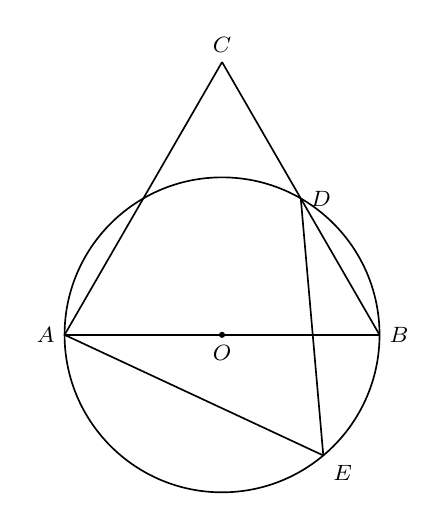
\begin{tikzpicture}[x=1cm, y=1cm, line width=0.6pt, font=\footnotesize]

  \coordinate (O)  at (0,0);
  \coordinate (A)  at (-2,0);
  \coordinate (B)  at (2,0);
  \coordinate (D)  at (1.00,1.732);
  \coordinate (C)  at (0,3.464);
  \coordinate (E)  at (1.286,-1.532);

  % ---------- 圆与直径 ----------
  \draw (0,0) circle (2);
  \draw (A) -- (B);

  % ---------- 题设线段 ----------
  \draw (B) -- (D) -- (C);
  \draw (A) -- (C);
  \draw (A) -- (E);
  \draw (D) -- (E);

  % ---------- 点与标注 ----------
  \fill (O) circle (1.1pt);
  \node[below]       at (O) {$O$};
  \node[left]        at (A) {$A$};
  \node[right]       at (B) {$B$};
  \node[right]       at (D) {$D$};
  \node[above]       at (C) {$C$};
  \node[below right] at (E) {$E$};

\end{tikzpicture}
\end{center}
\nopagebreak[4]
（2） 【B】已知矩阵 $\boldsymbol A$ 的逆矩阵 $\boldsymbol A^{-1}=\begin{bmatrix}-\dfrac14&\dfrac34\\[4pt]\dfrac12&-\dfrac12\end{bmatrix}$，求矩阵 $\boldsymbol A$ 的特征值。

（3） 【C】在极坐标系中，已知圆 $C$ 经过点 $P\left(\sqrt2,\dfrac\pi4\right)$，圆心为直线 $\rho\sin\left(\theta-\dfrac\pi3\right)=-\dfrac{\sqrt3}{2}$ 与极轴的交点，求圆 $C$ 的极坐标方程。

（4） 【D】已知实数 $x$，$y$ 满足：$|x+y|<\dfrac13$，$|2x-y|<\dfrac16$，求证：$|y|<\dfrac{5}{18}$。

\end{question}
\begin{question}
\gkti{22}设 $\xi$ 为随机变量，从棱长为 $1$ 的正方体的 $12$ 条棱中任取两条，当两条棱相交时，$\xi=0$；当两条棱平行时，$\xi$ 的值为两条棱之间的距离；当两条棱异面时，$\xi=1$。

（1） 求概率 $P(\xi=0)$；

（2） 求 $\xi$ 的分布列，并求其数学期望 $E(\xi)$。

\end{question}
\begin{question}
\gkti{23}设集合 $P_n=\{1,2,\cdots,n\}$，$n\in\mathbf N^*$。记 $f(n)$ 为同时满足下列条件的集合 $A$ 的个数：① $A\subseteq P_n$；② 若 $x\in A$，则 $2x\notin A$；③ 若 $x\in\complement_{P_n}A$，则 $2x\notin\complement_{P_n}A$。

（1） 求 $f(4)$；

（2） 求 $f(n)$ 的解析式（用 $n$ 表示）。

\end{question}